% This is the Reed College LaTeX thesis template. Most of the work
% for the document class was done by Sam Noble (SN), as well as this
% template. Later comments etc. by Ben Salzberg (BTS). Additional
% restructuring and APA support by Jess Youngberg (JY).
% Your comments and suggestions are more than welcome; please email
% them to cus@reed.edu
%
% See http://web.reed.edu/cis/help/latex.html for help. There are a
% great bunch of help pages there, with notes on
% getting started, bibtex, etc. Go there and read it if you're not
% already familiar with LaTeX.
%
% Any line that starts with a percent symbol is a comment.
% They won't show up in the document, and are useful for notes
% to yourself and explaining commands.
% Commenting also removes a line from the document;
% very handy for troubleshooting problems. -BTS

% As far as I know, this follows the requirements laid out in
% the 2002-2003 Senior Handbook. Ask a librarian to check the
% document before binding. -SN

%%
%% Preamble
%%
% \documentclass{<something>} must begin each LaTeX document
\documentclass[12pt,twoside]{reedthesis}
% Packages are extensions to the basic LaTeX functions. Whatever you
% want to typeset, there is probably a package out there for it.
% Chemistry (chemtex), screenplays, you name it.
% Check out CTAN to see: http://www.ctan.org/
%%
\usepackage{graphicx,latexsym}
\usepackage{amsmath}
\usepackage{amssymb,amsthm}
\usepackage{longtable,booktabs,setspace}
\usepackage{chemarr} %% Useful for one reaction arrow, useless if you're not a chem major
\usepackage[hyphens]{url}
% Added by CII
\usepackage{hyperref}
\usepackage{lmodern}
\usepackage{float}
\floatplacement{figure}{H}
% End of CII addition
\usepackage{rotating}

% Next line commented out by CII
%%% \usepackage{natbib}
% Comment out the natbib line above and uncomment the following two lines to use the new
% biblatex-chicago style, for Chicago A. Also make some changes at the end where the
% bibliography is included.
%\usepackage{biblatex-chicago}
%\bibliography{thesis}


% Added by CII (Thanks, Hadley!)
% Use ref for internal links
\renewcommand{\hyperref}[2][???]{\autoref{#1}}
\def\chapterautorefname{Chapter}
\def\sectionautorefname{Section}
\def\subsectionautorefname{Subsection}
% End of CII addition

% Added by CII
\usepackage{caption}
\captionsetup{width=5in}
% End of CII addition

% \usepackage{times} % other fonts are available like times, bookman, charter, palatino


% To pass between YAML and LaTeX the dollar signs are added by CII
\title{INFFOREST Variable Importance on Random Forests}
\author{Aurora Owens}
% The month and year that you submit your FINAL draft TO THE LIBRARY (May or December)
\date{May 2017}
\division{Mathematics and Natural Sciences}
\advisor{Andrew Bray}
%If you have two advisors for some reason, you can use the following
% Uncommented out by CII
% End of CII addition

%%% Remember to use the correct department!
\department{Mathematics}
% if you're writing a thesis in an interdisciplinary major,
% uncomment the line below and change the text as appropriate.
% check the Senior Handbook if unsure.
%\thedivisionof{The Established Interdisciplinary Committee for}
% if you want the approval page to say "Approved for the Committee",
% uncomment the next line
%\approvedforthe{Committee}

% Added by CII
%%% Copied from knitr
%% maxwidth is the original width if it's less than linewidth
%% otherwise use linewidth (to make sure the graphics do not exceed the margin)
\makeatletter
\def\maxwidth{ %
  \ifdim\Gin@nat@width>\linewidth
    \linewidth
  \else
    \Gin@nat@width
  \fi
}
\makeatother

\renewcommand{\contentsname}{Table of Contents}
% End of CII addition

\setlength{\parskip}{0pt}

% Added by CII

\providecommand{\tightlist}{%
  \setlength{\itemsep}{0pt}\setlength{\parskip}{0pt}}

\Acknowledgements{
.
}

\Dedication{
.
}

\Preface{

}

\Abstract{
Random forests are powerful predictive models but they lack a built-in
method for statistical inference. This paper compares several of the
most common methods of performing inference on random forests while
presenting a new method, INFFOREST variable importance. On simulated
data with multicollinearity, the INFFOREST method is able to show
significance for four out of five predictors used to generate the
response. Existing methods are tested and performed similarly on the
simulated data set. INFFOREST variable importance allows claims to be
made about the relationship between a predictor and the response, in the
context of the rest of the variables in the model. This sets it apart
from the exiting methods and creates some interesting implications.\par
}

	\usepackage{float}
\usepackage{amssymb,amsthm,amsmath}
\usepackage{chemarr}
\usepackage{algorithm}
\usepackage{algpseudocode}
\usepackage{pifont}
\usepackage{float}
\usepackage{tikz}

\let\origfigure\figure
\let\endorigfigure\endfigure
\renewenvironment{figure}[1][2] {
    \expandafter\origfigure\expandafter[H]
} {
    \endorigfigure
}
% End of CII addition
%%
%% End Preamble
%%
%

\begin{document}

% Everything below added by CII
      \maketitle
  
  \frontmatter % this stuff will be roman-numbered
  \pagestyle{empty} % this removes page numbers from the frontmatter

      \begin{acknowledgements}
      .
    \end{acknowledgements}
  
  
      \hypersetup{linkcolor=black}
    \setcounter{tocdepth}{2}
    \tableofcontents
  
      \listoftables
  
      \listoffigures
  
      \begin{abstract}
      Random forests are powerful predictive models but they lack a built-in
      method for statistical inference. This paper compares several of the
      most common methods of performing inference on random forests while
      presenting a new method, INFFOREST variable importance. On simulated
      data with multicollinearity, the INFFOREST method is able to show
      significance for four out of five predictors used to generate the
      response. Existing methods are tested and performed similarly on the
      simulated data set. INFFOREST variable importance allows claims to be
      made about the relationship between a predictor and the response, in the
      context of the rest of the variables in the model. This sets it apart
      from the exiting methods and creates some interesting implications.\par
    \end{abstract}
  
      \begin{dedication}
      .
    \end{dedication}
  
  \mainmatter % here the regular arabic numbering starts
  \pagestyle{fancyplain} % turns page numbering back on

  \chapter{Introduction}\label{introduction}
  
  \section{Trees and Random Forests}\label{trees-and-random-forests}
  
  To begin our discussion of trees and random forests, we will first
  consider the following example using data from a dendrologic study of
  five orange trees. This study measured two variables for each tree: the
  age of the tree (recorded in days) and the circumference of the trunk
  (in cm). These are called, in general terms, the variables recorded by
  the study. In the dataset below, each column represents a variable and
  each row represents one set of measurements. There are 2 columns (age
  and circumference) and 35 rows. The first six rows are displayed in
  table \ref{tab:taborange}.
  
  \begin{table}
  
  \caption{\label{tab:unnamed-chunk-2}\label{tab:taborange}The first six rows of the orange trees data set}
  \centering
  \begin{tabular}[t]{r|r}
  \hline
  age & circumference\\
  \hline
  118 & 30\\
  \hline
  484 & 58\\
  \hline
  664 & 87\\
  \hline
  1004 & 115\\
  \hline
  1231 & 120\\
  \hline
  1372 & 142\\
  \hline
  \end{tabular}
  \end{table}
  
  ~~~~~Let's pretend we are interested in the following question: knowing
  only the circumference of the orange tree, can we predict the age of the
  tree? This question can be translated into a formula. Formulas represent
  guesses of way the data was generated. We often refer to formulas using
  the following notation:
  
  \[Age \sim Circumference \]
  
  ~~~~~In this formula, circumference is the predictor and age is the
  response. Suppose we expanded the study to include the height of the
  orange trees at various stages of development. Now we can consider both
  the circumference and the height of the tree when we make our
  predictions of the age. When we have multiple predictors, we add them to
  the notation in the following way:\footnote{Often the notation for
    multiple predictors is written \(Y \sim X+W\) but this assumes an
    additive, linear relationship between the predictors and the response.
    This assumption is unnecessary for tree-based models so the notation,
    \(Y\sim X,W\) is used.}
  
  \[Age \sim Circumference, Height\]
  
  ~~~~~Returning to the original orange tree data set, we can begin to
  assess the structure in the data set by plotting the data and observing
  the relationship between the variables in figure
  \ref{fig:figOrangeTree1}.
  
  \begin{figure}[H]
  
  {\centering \includegraphics{Thesis_files/figure-latex/figOrangeTree1-1} 
  
  }
  
  \caption{The relationship between age and circumference of the trunk of orange trees.}\label{fig:figOrangeTree1}
  \end{figure}
  
  ~~~~~As can be seen in figure \ref{fig:figOrangeTree1}, generally older
  trees have thicker trunks, and it seems like we are not wrong to suspect
  that circumference is a good predictor of age. As the data could be
  reasonably represented by a straight line, we can say that the
  relationship between trunk circumference and tree age is roughly linear.
  Now that we have a formula, we can build a model to test it. To create
  our predictions of age, we fit the formula \(Age \sim Circumference\) to
  a model. A predictive model is, put simply, a systematic way to make our
  predictions. The most common type of model is the linear model, which
  creates predictions from a line through the data.
  
  \begin{figure}[htbp]
  \centering
  \includegraphics{Thesis_files/figure-latex/unnamed-chunk-3-1.pdf}
  \caption{\label{fig:unnamed-chunk-3}\label{fig:OrangeLM}A linear model
  representing age \textasciitilde{} trunk circumference in orange trees.
  The shaded area represents a 95\% confidence interval around this line.}
  \end{figure}
  
  ~~~~~As can be guessed from figure \ref{fig:OrangeLM}, the linear model
  works better on certain data than others. The linear model necessitates
  several assumptions that may not always be appropriate. We'll return to
  a brief discussion of the assumptions of the linear model later in this
  chapter.
  
  ~~~~~This paper discusses at length tree-based models. A tree for the
  formula \(age \sim circumference\) is similar to the linear model in
  that it presents a systematic way to make predictions, but the two
  differ in that the tree is not linear in any fashion. In fact, we can
  compare the differences between the two models by comparing figures
  \ref{fig:OrangeLM} and \ref{fig:orangeTreePartition}.
  
  \begin{figure}[H]
  
  {\centering \includegraphics{Thesis_files/figure-latex/unnamed-chunk-6-1} 
  
  }
  
  \caption{\label{fig:orangeTreePartition}A tree modeling the formula age \(\sim\)  trunk circumference first creates partitions on the predictor, seen as vertical lines, and then predicts the value of the response within that partition, seen as text.}\label{fig:unnamed-chunk-6}
  \end{figure}
  
  ~~~~~When using the linear model, we make predictions in the following
  way: given a value of X (circumference) the corresponding value of Y
  (age) on the line is our prediction. The predictions from the tree are
  gathered similarly: given a value of X (circumference), our prediction
  is the average value of Y (age) within the partition that X falls
  into.\footnote{While any curve can be approximated in a step-wise manner
    when the number of steps approaches \(\infty\), a tree model does not
    converge to the linear model as the number of splits approaches the
    number of observations, even when the data is linear.}
  
  ~~~~~Tree methods get their name from a common way of representing them
  in higher dimensions, when there is more than one predictor. Figure
  \ref{fig:figorangeTree} shows this method. In this case, given a new
  value for circumference, one would start their predictions at the top of
  the tree and, depending on the value of circumference and the
  instructions at each intersection or split, one would fall down branch
  by branch before landing on a prediction for age. If the new value for
  circumference is less than the value stated at the split, we would move
  down to the branch on the left. If circumference was more than the value
  for circumference at the split, we would move down to the branch on the
  right.
  
  \begin{figure}[H]
  
  {\centering \includegraphics{Thesis_files/figure-latex/unnamed-chunk-7-1} 
  
  }
  
  \caption{\label{fig:figorangeTree}A tree representing age \(\sim\) trunk circumference in orange trees.}\label{fig:unnamed-chunk-7}
  \end{figure}
  
  \subsection{Mathematical notation for
  trees}\label{mathematical-notation-for-trees}
  
  Given a data set, \(D\), and a formula \(Y \sim X\), where \(Y\) and
  \(X\) are columns in \(D\), a tree, \(t\), is a stepwise function from
  \(X\) to \(Y\). \(X\) can also be defined a a set of columns in \(D\).
  Recall, that \(X\) is the set of our predictors and \(Y\) is our
  response. In example in section 1.1, the orange trees data is the data
  set, the ages of the trees make up our response, and the circumferences
  are our predictor.
  
  \[t: X \rightarrow Y\] ~~~~~\(t\) is created using some sample of the
  rows of \(D\). This sample is called the \emph{training} set. The
  predictions or the image of \(t\), are discrete values in the range of
  \(Y\). We test the prediction accuracy of \(t\) using the rows of \(D\)
  that were not in the training set. This set of rows is called the
  \emph{test} set. Often with trees, we generate the training set from the
  initial data set \(D\) by \emph{bootstrapping} the \(D\).
  ``Bootstrapping'' means sampling with replacement. This allows us to
  have large test and training sets without starting with an extra large
  data set \(D\). This is valuable because it is more difficult to create
  good predictive models on small amounts of data relative to the entire
  population. The orange trees data set is an excelent candidate for
  bootstrapping, as there are only 35 records from 5 trees in the data set
  when there are presumably thousands of orange trees in the world at
  large. Table \ref{tab:tabbootorange} demonstrates a bootstrapped sample
  of the first six rows of the orange trees data set from table
  \ref{tab:taborange}.
  
  \begin{table}
  \caption{\label{tab:unnamed-chunk-9}\label{tab:tabbootorange}The first six rows of the orange trees data set are repeated here (left) with row numbers. The table on the right represent a bootstrapped sample of the data on the left.}
  
  \centering
  \begin{tabular}[t]{rrr}
  \toprule
  age & circumference & row\\
  \midrule
  118 & 30 & 1\\
  484 & 58 & 2\\
  664 & 87 & 3\\
  1004 & 115 & 4\\
  1231 & 120 & 5\\
  1372 & 142 & 6\\
  \bottomrule
  \end{tabular}
  \centering
  \begin{tabular}[t]{rrr}
  \toprule
  age & circumference & row\\
  \midrule
  484 & 58 & 2\\
  664 & 87 & 3\\
  1004 & 115 & 4\\
  1372 & 142 & 6\\
  484 & 58 & 2\\
  1372 & 142 & 6\\
  \bottomrule
  \end{tabular}
  \end{table}
  
  ~~~~~There are many ways to test prediction accuracy of a model, but we
  will be considering the following two in this paper: \(MSE\) and
  \(RSS\).\footnote{This paper considers only the case of regression with
    continuous random variables. There are analogous ways to test
    predictive accuracy for other types of data but they are beyond the
    scope of this paper.} \(MSE\) is the mean squared error and is defined
  as: \[MSE(t,Y,X) = \frac{1}{n} \sum_1^n (Y - t(X))^2\] Where \(n\) is
  the number of rows in \(X\) and \(Y\). \(RSS\) is the residual sum of
  squares error and is defined as: \[RSS(t,X,Y) = \sum_1^n (Y - t(X))^2\]
  
  ~~~~~In many cases, we are interested in creating predictive models to
  use as tools to predict the response in situations where an observed
  value is missing or difficult to find. We may want to build a model to
  predict the age of orange trees from trunk circumference because while
  it is relatively easy to measure the circumference of the trunk, age is
  often unknown. Then our model could be used to estimate the age of
  orange trees in situations where only circumference is known. When we
  generate predictions on new observations of the response, we cannot know
  how accurate our predictions are. Often \(MSE\) and \(RSS\) are
  calculated on the test set to create an estimate of how well the model
  will be able to predict the outcome of a new observation. Then they are
  refered to as \(MSE_{test}\) and \(RSS_{test}\), respectively.
  
  \subsection{A brief history of trees}\label{a-brief-history-of-trees}
  
  Trees are a convenient way to represent data and assist in decision
  making. Morgan and Sonquist (1963) derived a way for constructing trees
  motivated by the specific characteristics of data collected from
  interviews and surveys. The first difficulty in analyzing this data was
  that data collected from surveys is mostly categorical, where the
  observation is that the participant is a member of some discrete group.
  Some common categorical variables are gender, ethnicity, and education
  level. Numeric variables, like age, height, and weight are, in general,
  much easier to work with. On top of this, the data sets Morgan and
  Sonquist dealt with had few participants (rows) and many variables
  (columns). To add to their difficulties, there was reason to believe
  that there were lurking errors in the data that would be hard to
  identify and quantify. Lastly, many of the predictors were correlated.
  Morgan and Sonquist doubted that the additive assumptions of many models
  would be appropriate for this data. They noted that while many
  statistical methods would have difficulty accurately parsing this data,
  a clever researcher with quite a lot of time could create a suitable
  model simply by grouping values of the predictors and predicting that
  the response corresponding to these values would be an average of the
  observed responses given the grouped conditions. Their formalization of
  this procedure in terms of ``decision rules'' laid the groundwork for
  future research on decision trees.(Venables \& Ripley, 2002) See figure
  \ref{fig:orangeTreePartition} for a visualization of this process.
  
  ~~~~~Later researchers proposed new methods for creating trees that
  improved upon the Morgan and Sonquist model. Leo Breiman et al. proposed
  an algorithm called CART (Classification And Regression Trees) to fit
  trees on various types of data (1984). Torsten Hothorn, Kurt Hornik and
  Achim Zeileis argue in their 2006 paper, \emph{Unbiased Recursive
  Partitioning: A Conditional Inference Framework}, CART has a selection
  bias toward variables with either missing values or a great number of
  possible splits. This bias can affect the interpretability of all tree
  models fit using this method. As an alternative to CART and other
  algorithms, Hothorn et al. propose a new method: conditional inference
  trees. The conditional inference trees algorithm is similar to CART in
  many ways, but a thourough description is beyond the scope of this
  paper.
  
  ~~~~~In the 1984 textbook \emph{Classification and Regression Trees},
  Breiman, Friedman, Olshen, and Stone described their method for
  creating, pruning, and testing regression trees. There are essentially
  three steps: one, decide on a variable to split over, two, partition
  that variable space in two distinct partitions, and three, set our
  initial predictions for each partition to be mean value of the response
  according to the observed responses corresponding to the values in the
  partitions. Recursively, this process is repeated for each new partition
  until some stopping condition is reached. This is a top down, greedy
  algorithm that functions by creating as large a tree as possible
  (Venables \& Ripley, 2002).
  
  ~~~~~Random Forests are generated by fitting a large number of trees,
  each on a boosted sample of the data. The crucial difference, however,
  between the trees in CART and the trees in a random forest, is that at
  each node in a random forest, only a subset of the predictors are
  considered as candidates for possible splits. This decorrelates each
  tree from its neighbors, and limits variability of the whole forest
  (James, Witten, Hastie, \& Tibshirani, 2013).
  
  ~~~~~ There is a limit to the predictive capabilities of a single tree
  as they suffer from high variance. (James et al., 2013) These are
  further explored in chapter 2. To alleviate this, aggregate methods
  called forests are often used instead. They function by enlisting the
  help of many trees, and then by aggregating the responses over all of
  them. The two common types of forests are bagged and random forests.
  
  \subsection{Mathematical notation for bagged and random
  forests}\label{mathematical-notation-for-bagged-and-random-forests}
  
  Given a data set, \(D\), and a formula \(Y \sim X\), where \(Y\) and
  \(X\) are columns in \(D\), a forest, \(R\), collection of trees from
  \(X\) to \(Y\). As \(R\) is a collection of trees from \(X\) to \(Y\),
  it is also a stepwise function from \(X\) to \(Y\).
  
  \[R:X \rightarrow Y\]
  
  The trees in a forest are fit using bootstrapped samples of the original
  data set \(D\). The bootstrapped training set for a tree \(t\) is
  \(B_t\) and the corresponding test set is \(\bar{B}_t\). These test and
  training sets are called the \emph{in bag} set and the \emph{out of bag}
  set. When the \(MSE\) or \(RSS\) is calculated for a tree in a forest,
  it is done on the out of bag set for that tree and called the OOB (out
  of bag) error. The predictive accuracy of the random forest is the
  average of the out of bag error across all the trees in the forest. The
  predictions for the random forest, \(R(X)\), are the average prediction
  of each tree on \(X\).
  
  These are \emph{bagged forests}. \emph{Random forests} are a variation
  on bagged forests, and the main focus of this paper. There is no
  difference between bagged and random forests when there is only one
  predictor in the data set, but, in cases with more than one predictor,
  the trees are generated in a slightly different way. Usually, to make a
  split all the predictors are considered. (Recall that splits are rules
  on certain predictors; rules like ``if circumference is less than 113.5
  go left, if not go right.'' The statement ``circumference \textless{}
  113.5'' from figure \ref{fig:figorangeTree} is a split at 113.5 on the
  variable circumference). If we had a larger version of the orange tree
  data set that included the heights of each tree, then the tree would
  always consider both height and circumference as possible candidates for
  splits. In a random forest on this expanded orange tree data set, it is
  possible that only one predictor, height or circumference, would be
  considered at a time. The splitting procedure is discussed at length in
  chapter 3 and this property of random forests is discussed in chapter 4.
  For now only a cursory understanding is needed.
  
  \subsection{Inferential vs Descriptive
  Statistics}\label{inferential-vs-descriptive-statistics}
  
  In the earlier sections, we focused on building predictive models, but
  this paper hopes to use tree-based methods beyond this context. The
  linear model is a mainstay in social science because it allows for easy
  and interpretable statistical inference. Return to the orange tree
  example from section 1.1. The linear model gives us a line with which we
  can make predictions, but it also gives estimated coefficients and
  conducts hypothesis tests on the values of the coefficients.
  
  \begin{table}
  
  \caption{\label{tab:unnamed-chunk-11}\label{tab:tablmcoef}Estimated linear coefficients, error, and p-values from the model fit in section 1.1 on the orange tree dataset}
  \centering
  \begin{tabular}[t]{l|r|r|r|r}
  \hline
    & Estimate & Std. Error & t value & Pr(>|t|)\\
  \hline
  (Intercept) & 16.603609 & 78.1406182 & 0.2124837 & 0.8330368\\
  \hline
  circumference & 7.815998 & 0.6058806 & 12.9002281 & 0.0000000\\
  \hline
  \end{tabular}
  \end{table}
  
  This table provides evidence that not only is trunk circumference a good
  predictor of age, the relationship between them is the equation of the
  line:
  
  \[Age = 7.81 \cdot Circumference + 16.6\]
  
  ~~~~~Roughly, for every 1 cm of trunk growth, we would expect the tree
  to be 7.81 days older. Not only are we provided with a way to describe
  the relationship between age and circumference, we have conducted
  statistical tests to make reasonably sure that our estimates, 7.81 and
  16.6 in the equation above, are not zero. Inferential claims about the
  nature of tree age and trunk growth are possible here.
  
  ~~~~~It is important to note the difference between inferential and
  descriptive statistics. Descriptive statistics describe the data at hand
  without making any reference to a larger data generating system that
  they come from. It follows that inferential statistics then make claims
  about the data generating system given the data. The model in figure
  \ref{fig:figorangeTree} could be used to make descriptive claims about
  the orange tree data. For example, given the data we have, we expect a
  sapling with a trunk circumference less than 41 cm to be 118 days old.
  However, trees are variable; they are very sensitive to changes in the
  data set. It's entirely possible that if we fit this tree on a new
  sample of the data, the predictions would change. See chapter 2 for more
  discussion on the variability of trees. Our claims about the relation
  between circumference and age in young orange trees can only be
  descriptive as we have not taken into account the variability in
  gathering them. This paper's aim is to describe a process of making
  inferential claims using trees and random forests that employs
  permutation tests.
  
  ~~~~~As stated in the introduction of the \emph{Chronicle of
  Permutations Statistical Methods} by KJ Berry et al. 2014, there are two
  models of statistical inference. One is the population model, where we
  assume that the data was randomly sampled from one (or more)
  populations. Under this model, we assume that the data generated follows
  some known distribution. ``Under the population model, the level of
  statistical significance that results from applying a statistical test
  to the results of an experiment or a survey corresponds to the frequency
  with which the null hypothesis would be rejected in repeated random
  samplings from the same specified population(s)'' (Berry, 2014).
  
  ~~~~~The permutation family of methods, on the other hand, only assumes
  that the observed result was caused by experimental variability. The
  test statistics are calculated for the observed data, then the data is
  permuted a number of times. The statistic is calculated after each
  permutation to derive a distribution of possible values under some null
  hypothesis. Then the original test statistic is tested against this
  distribution. If the observed value is exceptionally rare, then there is
  evidence that our observation did not come from that distribution.
  
  \section{Inference on Random Forests}\label{inference-on-random-forests}
  
  \subsection{The Problem}\label{the-problem}
  
  Random forests create models with great predictive, but poor inferential
  capabilities. After Morgan and Sonquist's initial development of
  decision trees, trees quickly moved to the domain of machine learning
  and away from statistics. Researchers focused on bettering predictions
  and improving run times and less on the statistics behind them. In a
  single tree, descriptive claims may be simple to make, but it is much
  more difficult to describe the behavior of the whole forest. Inferential
  statistics with random forests generally falls behind the predictions in
  importance. This has limited the applications of random forests in
  certain fields, as to many the question of ``why'' the data is the way
  it is is more important than building predictions. There are several
  means of performing descriptive statistics with random forests that
  could be interpreted incorrectly as attempting to answer this but
  without a statistically backed method for performing inference, the use
  of random forest is limited to prediction-only settings.
  
  \subsection{Proposed solutions to this
  problem}\label{proposed-solutions-to-this-problem}
  
  Variable importance could be the tree-based analogue to the coefficients
  of the linear model, in that the variable importance for the predictor
  \(X_i\) in the model for \(Y \sim X_1,...,X_p\) is the amount of
  predictive accuracy due to \(X_i\). Breiman proposed a method of
  permuted variable importance in his paper \emph{Statistical Modeling:
  The Two Cultures} to answer this problem. Their method compares the
  variable importance for each variable in a tree-wise manner. For each
  tree, the permuted variable importance of the variable \(X_j\) is:
  
  \[VI^t(X_j) = \frac{\sum_{i \in |\bar{B}_t|} ({y} - \hat{y})^2}{|\bar{B}_t|} - \frac{\sum_{i \in |\bar{B}_t^*} ({y} - \hat{y}^*)^2}{|\bar{B}_t^*|} \]
  
  ~~~~~ Where \(\bar{B}^t\) is the out of bag sample for tree t, \(|B|\)
  is the number of observations in that sample, \(\bar{B}_p^t\) is with
  \(X_j\) permuted, \(\hat{y}\) is the predicted outcome, and
  \(\hat{y}^*\) is the predicted outcomes after variable \(X_j\) has been
  permuted. This value is averaged over all the trees. It is important to
  note that if the variable \(X_j\) is not split on in the tree \(t\), the
  tree-wise variable importance will be 0.
  
  ~~~~~ Strobl et al from the University of Munich criticize this method
  in their 2008 technical report \emph{Danger: High Power! -- Exploring
  the Statistical Properties of a Test for Random Forest Variable
  Importance}. First, this method has the downside of increasing power
  with increasing numbers of trees in the forest. This is a more or less
  arbitrary parameter which we would hope would not affect our importance
  estimates. Second, the null hypothesis under Breiman and Cutler's
  strategy is that the variable importance \(VI\) for any variable \(X_j\)
  is not equal to zero given \(Y\), the response. Because random forests
  are most often used in situations with multicolinearity that would make
  other methods like the linear model difficult, Strobl argues that any
  variable importance measure worth its salt should not be misled by
  correlation within the predictors.
  
  ~~~~~ The researchers at the University of Munich published a fully
  fleshed response to the Breiman and Cutler method in 2008, titled
  \emph{Conditional Variable Importance for Random Forests} that addresses
  these issues. Strobl et al propose restructuring the Breiman and Cutler
  algorithm to account for conditional dependence among the predictors.
  The null hypothesis is that \(VI_{\beta}(X_j) = 0\) given the predictor
  \(Y\) \emph{and all other predictors} \(X_1,..X_n\). This accounts for
  interactions between \(X_j\) and the other predictors, while preserving
  the relationship between \(Y\) and the remaining predictors.
  
  ~~~~~This paper aims to provide a response to this method. The
  partitions are made from the random forest corresponding to the formula
  of \(Y \sim X_1,...,X_n\) instead of a model of
  \(X_j \sim X_1,...,X_n\). This ignores the common situation where if the
  predictors are correlated enough, then they act as stand ins for each
  other, so that if one variable is heavily influential in a certain tree
  at predicting \(Y\), the other variable will be forgotten altogether.
  
  \chapter{Simulations and Comparisons}\label{simulations-and-comparisons}
  
  Our goal for this chapter is to compare trees, random forests, and
  linear models. In this chapter, we will use simulated data instead of
  the orange trees data set. One reason for this is theoretical
  consistency. One hopes that one's results will not be rendered null and
  void by any misstep in the data collection that comes to light. This
  also ensures that these simulations can be repeated by later
  researchers, but, granted, it does not make for the most exciting
  analysis. For now, consider \(Y\) to be our response variable. In the
  first simulation, \(V\) will be the set of our predictors, and \(V_j\)
  to be a predictor in \(V\). The formula will be the same for each model:
  \(Y \sim V\). In our second simulation, our set of predictors will be
  denoted as \(X\) and \(X_j\) will be a member of \(X\). The formula in
  this case is \(Y \sim X\). A single row in \(D_1\) will be denoted as
  \(v\), and a single row in \(D_2\) as \(x\).
  
  \section{Simulated Data}\label{simulated-data}
  
  Random forests excel in predicting outcomes with correlated predictors,
  although these situations can make it difficult to perform intelligible
  inference. In a situation in which the correlated predictors are \(X_1\)
  and \(X_2\) and the formula we're estimating is \(Y \sim X_1 + X_2\), it
  can be difficult to say if \(X_1\) or \(X_2\) is truly the better
  predictor. To illustrate this idea, compare a few existing methods, and
  explore methods of inference on tree based models, we will simulate two
  data sets with different correlation structures. We will focus more on
  the correlation structure between the predictors than on their
  relationships with the response and this will be reflected in the
  simulations.
  
  ~~~~~The first simulated dataset is generated under the same scheme as
  in (Strobl, Boulesteix, Kneib, Augustin, \& Zeileis, 2008). Under this
  method, the 13 x 1000 data set, \(D_1\), has 12 predictors,
  \(V_1,..,V_{12}\), where \(V_j \sim N(0,1)\). The first four are block
  correlated to each other with \(\rho = .9\). They are related to \(Y\)
  by the linear equation:
  \[Y = 5 \cdot V_1 + 5 \cdot V_2 + 2 \cdot V_3 + 0 \cdot V_4 + -5 \cdot V_5 + -5\cdot V_6 + 0\cdot V_7 + 0 \cdot ..... + E, E \sim N(0,\frac 1 2 )\]
  Note in table \ref{tab:tabcorSim1}, the coefficients for
  \(V_7,...,V_{12}\) are all zero.
  
  \begin{table}
  
  \caption{\label{tab:unnamed-chunk-12}\label{tab:tabcorSim1}Empirical correlations and coefficients of the variables in the first simulated data set}
  \centering
  \begin{tabular}[t]{l|r|r|r|r|r|r|r|r|r}
  \hline
    & V1 & V2 & V3 & V4 & V5 & V6 & V7 & y & beta\\
  \hline
  V1 & 1.000 & 0.915 & 0.908 & 0.907 & -0.034 & 0.006 & 0.012 & 0.839 & 5\\
  \hline
  V2 & 0.915 & 1.000 & 0.914 & 0.914 & -0.020 & -0.001 & -0.001 & 0.838 & 5\\
  \hline
  V3 & 0.908 & 0.914 & 1.000 & 0.903 & -0.017 & -0.007 & 0.007 & 0.818 & 2\\
  \hline
  V4 & 0.907 & 0.914 & 0.903 & 1.000 & -0.002 & -0.015 & 0.023 & 0.800 & 0\\
  \hline
  V5 & -0.034 & -0.020 & -0.017 & -0.002 & 1.000 & 0.044 & 0.005 & -0.392 & -5\\
  \hline
  V6 & 0.006 & -0.001 & -0.007 & -0.015 & 0.044 & 1.000 & -0.005 & -0.368 & -5\\
  \hline
  V7 & 0.012 & -0.001 & 0.007 & 0.023 & 0.005 & -0.005 & 1.000 & 0.004 & 0\\
  \hline
  \end{tabular}
  \end{table}
  
  ~~~~~In the last column of table \ref{tab:tabcorSim1}, the coefficient
  ``beta'', refers to the function used to generate the \(Y\) values.
  Although \(V4\) was not included in the model \(Y \sim V1,..V_{12}\),
  its strong correlation with more influential predictors \(V_1,...,V_3\)
  ensures that it still shows a strong, empirical linear correlation with
  \(Y\). A linear model would likely \emph{overstate} the effect of
  \(V_4\) on \(Y\).\footnote{A brief note on uncertainty is needed here.
    It's true that in this setting we can say that \(V_4\) is actually
    unimportant to understanding \(Y\), but in situations with real data
    this is profoundly more difficult to parse. Often like in the social
    science situations that Morgan and Sonquist encountered, the real
    relationship between correlated predictors is complicated and often
    there is some theoretical backing or other insight that is gained to
    include variables that may not be important to the model.}\footnote{Another
    point that could be said is that, no \(V_4\) is not unimportant,
    \(V_1, V_2,\) and \(V_3\) are just stand ins for the real star,
    \(V_4\), as they are nearly the same (\(\rho \sim 1\)). Then the real
    relationship represented here is
    \(Y \sim (5 + 5 + 2) \cdot V_4 + -5 \cdot V_5 + -5 \cdot V_6 + -2 \cdot V_7\).
    This model is not unsuccessful in capturing the structure of the data,
    and this is typically the practice used to model data with highly
    correlated predictors. If this seems philosophically satisfying to
    you, the rest of this thesis may seem a bit inconsequential.}
  
  \begin{figure}[htbp]
  \centering
  \includegraphics{Thesis_files/figure-latex/figdenv4y-1.pdf}
  \caption{\label{fig:figdenv4y}Relation between V4 and Y. This relation has
  empirical linear correlation = .789}
  \end{figure}
  
  \begin{figure}[htbp]
  \centering
  \includegraphics{Thesis_files/figure-latex/unnamed-chunk-14-1.pdf}
  \caption{\label{fig:unnamed-chunk-14}\label{fig:figdenv1v5}Empirical
  densities for V1 through V4}
  \end{figure}
  
  ~~~~~The densities of \(V_1,...,V_4\) in figure \ref{fig:figdenv1v5} are
  all very similar due to the way they were generated. \(D_1\) represents
  the case where some of the predictors are linearly correlated with each
  other, but that is not the only possible correlation structure. The data
  set \(D_2\) is simulated similarly to \(D_2\) in that \(D_2\) contains
  twelve predictors and one response variable. The first four variables
  are generated in the following way: \[X_1 \sim N(0,1)\]
  \[X_2 = log(X_1) + E, E \sim N(0,1)\]
  \[X_3 = log(X_2) + E, E \sim N(0,1)\]
  \[X_4 = log(X_4) + E, E \sim N(0,1)\]
  
  This simulation scheme leads to the first four variables having an
  obvious relationship between each other, but relatively low linear
  correlations, as seen in figure \ref{fig:corstructd2}. Predictors are
  sampled by \(X_5,...,X_{12} \sim N(0,1)\). The \(Y\) values are
  generated according to the following formula:
  
  \[Y = 5 \cdot (X_1)^2 + 5 \cdot(X_2)^2 + 2 \cdot (X_3)^2 + 0 \cdot X_4 + -5 \cdot X_5 + -5\cdot X_6 + 0\cdot X_7 + 0 \cdot ..... + E, E \sim N(0,\frac 1 2 )\]
  
  \begin{figure}[htbp]
  \centering
  \includegraphics{Thesis_files/figure-latex/unnamed-chunk-15-1.pdf}
  \caption{\label{fig:unnamed-chunk-15}\label{fig:corstructd2}Correlation
  structure of the first four variables in D2}
  \end{figure}
  
  ~~~~~The correlation structure in \(D_2\) is much more difficult to
  capture with a single line. The relationships between the first four
  predictors form striking, symmetrical scatter plots in figure
  \ref{fig:corstructd2}. This information is considered again in table
  \ref{tab:tabcorSim2}, where the empirical correlations of the first
  seven variables are presented along with their observed correlations
  with \(Y\) and their simulation coefficients.
  
  \begin{table}
  
  \caption{\label{tab:unnamed-chunk-17}\label{tab:tabcorSim2}Empirical correlations and coefficients of the first seven predictors and the response using the second simulated dataset}
  \centering
  \begin{tabular}[t]{l|r|r|r|r|r|r|r|r|r}
  \hline
    & X1 & X2 & X3 & X4 & X5 & X6 & X7 & y & beta\\
  \hline
  X1 & 1.000 & 0.013 & 0.044 & 0.002 & -0.012 & -0.012 & -0.044 & -0.003 & 5\\
  \hline
  X2 & 0.013 & 1.000 & -0.520 & -0.272 & 0.073 & 0.004 & 0.006 & -0.697 & 5\\
  \hline
  X3 & 0.044 & -0.520 & 1.000 & -0.004 & 0.030 & -0.013 & 0.023 & 0.271 & 2\\
  \hline
  X4 & 0.002 & -0.272 & -0.004 & 1.000 & -0.031 & 0.022 & -0.002 & 0.352 & 0\\
  \hline
  X5 & -0.012 & 0.073 & 0.030 & -0.031 & 1.000 & 0.010 & -0.030 & -0.099 & -5\\
  \hline
  X6 & -0.012 & 0.004 & -0.013 & 0.022 & 0.010 & 1.000 & -0.088 & -0.022 & -5\\
  \hline
  X7 & -0.044 & 0.006 & 0.023 & -0.002 & -0.030 & -0.088 & 1.000 & 0.013 & 0\\
  \hline
  \end{tabular}
  \end{table}
  
  \section{Models and Comparisons}\label{models-and-comparisons}
  
  \subsubsection{CART: Regression Trees}\label{cart-regression-trees}
  
  \begin{figure}[htbp]
  \centering
  \includegraphics{Thesis_files/figure-latex/unnamed-chunk-19-1.pdf}
  \caption{\label{fig:unnamed-chunk-19}\label{fig:figcarts}CART representing
  Y\textasciitilde{} X, from D2}
  \end{figure}
  
  The CART tree representing the model \(Y \sim X\) in figure
  \ref{fig:figcarts} is easy enough to understand. Starting at the very
  top of the tree, predictions can be made based on the values of the
  leaves (or ending nodes) given the requirements of the path to get
  there. Trees can be quite variable, so to get a better idea of the
  differences between the methods let's run a simulation. This simulation
  scheme will take advantage of the non linearity present in \(D_2\).
  
  \begin{algorithm}
  \caption{Simulation Scheme 2.1}
  \label{sim2.1}
  \begin{algorithmic}[1]
  \For{$i \leq 1000$ }
  \State Randomly sample $\frac 2 3$  of the observations in  $D_2$  to a training set,  $D_{2, train}^i$. The other observations,  $x \in D_2, x \notin D_{2, train}^i$ form the testing set $D_{2, test}^i$
  \State Fit a tree, $T^i$, to the data under the model $Y \sim X_1,...,X_2$ using the observations in $D_{2}^i$
  \State Calculate the $MSE_{test}$ of the model using the equation:
      $MSE_{test} = \frac 1 n \sum (y_j - \hat{y_j})^2$
  \EndFor
  \end{algorithmic}
  \end{algorithm}
  
  Note that \(n\) is the number of observations in \(D_{1, test}^i\),
  \(y_j \in D_{2, test}^i, \hat{y_j} \in T^i(D_{2, test}^i)\) for
  \(1 \leq j \leq n\) This produces one distribution of \(MSE_{test}\) for
  CART. This simulation scheme will be repeated for the linear model and
  the random forest and the \(MSE_{test}\) distributions are compared in
  figure \ref{fig:baggedvcartvforest}.\footnote{Recall that we only allow
    splits to take place that split the data into two groups, each with
    more than five members.} Note that the scales on the x-axis are
  drastically different for each of these models. The \(MSE_{test}\)
  distribution for the random forest has such low variance, and low
  \(MSE_{test}\) it would be difficult to display it on the same plot as
  the other two.
  
  \begin{figure}[htbp]
  \centering
  \includegraphics{Thesis_files/figure-latex/unnamed-chunk-20-1.pdf}
  \caption{\label{fig:unnamed-chunk-20}\label{fig:baggedvcartvforest}The
  simulated MSE distributions of CART, linear model, and the random forest
  on D2}
  \end{figure}
  
  ~~~~~The linear model is characteristically less flexible and less prone
  to over-fitting than either of the tree-based methods, CART and random
  forests, and has a \(MSE_{test}\) distribution that is quite peaked.
  CART is flexible and suffers from high variance. The random forest
  models perform much better on average than either the CART or the linear
  model, due to both the non-linear relationships between \(Y\) and the
  predictors and the random forest's ability to decorrelate each of the
  trees by restricting the variables available on each split. See chapter
  3 for more discussion on the enforced heterogeneity of trees in the
  random forest. As \(MSE_{test}\) is a test of \emph{predictive} accuracy
  it is not surprising that the random forest performed admirably. On a
  certain level, that is what they are designed to do. Highly predictive
  models are good at \emph{predicting} outcomes, but not necessarily good
  evidence that the data was generated in a similar way to that model. The
  linear model is not always popular in predictive situations but it is
  ubiquitous in inferential ones.
  
  \chapter{Random Forest Variable
  Importance}\label{random-forest-variable-importance}
  
  To implement the various variable importance measures discussed in this
  chapter and in chapter 4, functions for creating trees, random forests,
  and their importance measures were created. The trees were fit using the
  standard two-part CART-like algorithm. The function chooses a variable
  to split on with linear correlation with respect to \(Y\), but instead
  of looking for correlations above a certain threshold which is common,
  it chooses the variable with the highest correlation when compared to
  its peers. This alleviates the situation where a variable with a
  non-linear relationship would be passed over again and again. The
  splitting is then done via minimization of the following function with
  respect to \(i\):
  
  \[RSS_{node} (i,X,Y) = RSS_{leaf}(Y|X <i) + RSS_{leaf}(Y|X \geq i) \]
  \[RSS_{leaf} = \sum_{y \in Y} (y - \hat{y})^2 \]
  
  ~~~~~Note that \(\hat{y}\) is the mean value of \(Y\). This function
  considers the regression case only, and only numeric predictors. Leaves
  are created when the resultant split would be unsatisfactory, i.e.~at
  least one of these cases applies: one daughter node would have five
  members or less, the split on the chosen variable would not result in a
  decrease in RSS, or the response contained in the node, or the predictor
  considered for the split, are already homogeneous. This generates very
  large trees: a quality that is not an issue in random forests but may be
  problematic in a single-tree setting.
  
  \begin{table}
  
  \caption{\label{tab:unnamed-chunk-22}\label{tab:tabhomegrowntree}t, a home-grown tree grown on the first four columns and the first 140 rows of D2}
  \centering
  \begin{tabular}[t]{l|l|r|r|r}
  \hline
  var & n & dev & ypred & split.cutleft\\
  \hline
  X2 & 140 & 234791.36 & 49.79 & -4.52\\
  \hline
  X4 & 127 & 92293.01 & 33.49 & 0.64\\
  \hline
  X4 & 60 & 59974.42 & 49.64 & 3.86\\
  \hline
  leaf & 6 & 4827.51 & 96.24 & 0.00\\
  \hline
  X3 & 54 & 39569.87 & 44.46 & 1.91\\
  \hline
  leaf & 21 & 21874.78 & 65.75 & 0.00\\
  \hline
  leaf & 33 & 17695.09 & 30.91 & 0.00\\
  \hline
  X3 & 67 & 12473.55 & 19.03 & 1.45\\
  \hline
  leaf & 7 & 2562.75 & 45.24 & 0.00\\
  \hline
  X3 & 60 & 7608.15 & 15.97 & -0.18\\
  \hline
  X2 & 32 & 4033.15 & 21.77 & 1.05\\
  \hline
  leaf & 10 & 1486.19 & 31.31 & 0.00\\
  \hline
  leaf & 22 & 2546.96 & 17.43 & 0.00\\
  \hline
  X2 & 28 & 1678.22 & 9.35 & -0.47\\
  \hline
  leaf & 13 & 631.76 & 14.20 & 0.00\\
  \hline
  X2 & 15 & 660.31 & 5.15 & -0.88\\
  \hline
  leaf & 6 & 330.90 & -1.07 & 0.00\\
  \hline
  leaf & 9 & 329.41 & 9.29 & 0.00\\
  \hline
  leaf & 13 & 112843.76 & 208.98 & 0.00\\
  \hline
  \end{tabular}
  \end{table}
  
  ~~~~~There are several ways to display a tree, but when it is displayed
  as in table \ref{tab:tabhomegrowntree} it is read in the following way:
  each row corresponds to a node of the tree which contains a certain
  number, \texttt{n} observations. This number of observations, or rows in
  the data set is naturally a subset of both the original data set and the
  subsets above the node on the tree. Here our predictions,
  \texttt{ypred}, are the mean of the \(Y\) values included in the node.
  If there is an optimal and allowable split,\footnote{Recall that we only
    allow splits to take place that split the data into two groups, each
    with more than five members.} then the chosen variable, \texttt{var},
  and the \(RSS_{node}\), \texttt{dev}, are recorded.\footnote{It's the
    convention to call the \(RSS_{node}\) the deviance at a node \(N\),
    but, of course, this only makes sense when the node is a leaf.} The
  value of the variable in question that acts as the split point is
  recorded as \texttt{split.cutleft}. If there is no split on the node in
  question, then \texttt{var} will be recorded as
  \texttt{\textless{}leaf\textgreater{}} and the \texttt{dev} value will
  be the value of \(RSS_{leaf}\) at this node.
  
  ~~~~~The tree output is read roughly from top to bottom, with a coda in
  the middle. The first row corresponds to the first node, or the node
  that includes the entire data set. The second row is the beginning of
  the right subtree or the right daughter of the first node. This pattern
  continues, favoring the right daughter, until a leaf is reached. The
  left daughter of the first node is found after all of the splits off of
  the right daughter have finished but is easily identified as the row
  with a value of \texttt{n} that is exactly the difference between the
  \texttt{n} values of the first two rows. In the case where the right
  daughter contained many more observations of the original data set,
  there may be a node within the right subtree that contains the same
  number of observations as the left daughter of the first node.\footnote{This
    occurs when the variable in question has a group of values that are,
    1) larger in magnitude than the mean, and 2) are seperated from the
    general trend. Essentially this occurs when we have unscaled data with
    outliers.} In this case, the left daughter is simply the second row
  with this property. The pattern of following the right daughter until a
  leaf is reached continues with the left subtree.
  
  \section{Breiman et al. Introduce Permuted Variable Importance
  (1984)}\label{breiman-et-al.-introduce-permuted-variable-importance-1984}
  
  \subsection{Variable Importance on a Single
  Tree}\label{variable-importance-on-a-single-tree}
  
  Breiman et al. in \emph{Classification and Regression Trees} (1984)
  propose a method for variable importance for individual trees that stems
  from their definition of \(\tilde{s}\), a surrogate split. Surrogate
  splits help Breiman et al. deal with several common problems: missing
  data, masking, and variable importance. They are defined using logic
  that resembles that behind random forests.
  
  ~~~~~Before we discuss surrogate splits, let's cover an obvious
  definition of variable importance for a single tree. In the tree
  represented by table \ref{tab:tabhomegrowntree}, define variable
  importance as the number of splits on each variable. This would allow us
  to answer the question: how useful (important) was variable \(X_i\) in
  constructing our model for \(Y\)? Just by counting the splits on that
  variable, we would arrive at the following ranking:
  
  \begin{table}
  
  \caption{\label{tab:unnamed-chunk-24}\label{tab:tabbvi}The number of splits on each variable in the tree T.}
  \centering
  \begin{tabular}[t]{l|r}
  \hline
  variable & appearances.in.tree\\
  \hline
  X2 & 4\\
  \hline
  X3 & 3\\
  \hline
  X4 & 2\\
  \hline
  X1 & 0\\
  \hline
  \end{tabular}
  \end{table}
  
  ~~~~~There are several downfalls to this method. One, trees are
  variable. If we were to resample this data and fit another tree, it's
  likely that this ranking would change. Two, in the case where two
  variables are close enough to each other that they could act as
  stand-ins for one another, these rankings are much less interesting. We
  are lucky in this case to know without doubt that \(X_1\) has a rich
  relationship with \(X_2\) and the other predictors included in this
  model (see chapter 2, section 1). This leads us to believe that while
  \(X_1\) is left out of these rankings, it just as easily could have been
  included instead of \(X_2\), or one of the other predictors. \(X_1\) had
  bad luck by not being in this model and it wouldn't make sense to say
  that the \(X_1\) is the least important predictor of \(Y\) when it is
  very nearly identical to \(X_2\). However, it's possible that the tree
  algorithm would only pick one of the correlated predictors to be
  included in a model at a time. Is it possible that we can grasp this
  relationship by only fitting one tree?
  
  ~~~~~This dilemma is solved by surrogate splits. To set the stage for
  surrogate splitting, imagine a CART tree, \(t\), fit on some data set
  \(D\) according to the formula \(Y \sim X\) where
  \(X_i \in X, \\ if \\ i \in 1:p\). Now say that we're only considering a
  single node, \(N\), in \(t\). The node \(N\) contains the subset of the
  rows in the original data set \(D\), \(D_N\). \(D_N\) is determined by
  the previous nodes and splits in the tree.
  
  \begin{center}
  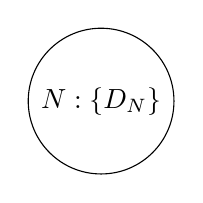
\begin{tikzpicture}[level/.style={sibling distance=60mm/#1}]
  \node [circle,draw] (z){$N:\left\{ D_N \right\}$};
  \end{tikzpicture}
  \end{center}
  
  ~~~~~On that node, we have the split on \(X_j\) where \(X_j < a\). This
  gives us two daughter nodes to \(N\), \(N_L\) and \(N_R\).
  
  \usetikzlibrary{positioning}
  
  \begin{center}
  \begin{tikzpicture}[level/.style={sibling distance=60mm/#1}]
  \node [circle,draw] (z) {$N:\left\{ D_N, \left\{X_j < a \right\}\right\}$};
  \node [circle,draw] (a) [below left = of z] {$N_L:\left\{ D_{N_L} \right\}$};
  \node [circle,draw] (b) [below right = of z] {$N_R:\left\{ D_{N_R} \right\}$};
  \end{tikzpicture}
  \end{center}
  
  ~~~~~The data sets \(D_{N_L}\) and \(D_{N_R}\) are subsets of \(D_N\)
  and when combined, they equal \(D_N\). They are determined by the rule:
  if a row of observations has a value of \(X_j < a\) then it is a member
  of \(D_{N_L}\), if the value of \(X_j\) in that row is greater than or
  equal to \(a\) then it belongs to \(D_{N_R}\). \(X_j\) was chosen to
  split on in node \(N\) because the correlation between the subsets of
  \(X_j\) and \(Y\) in \(D_N\) was stronger than the correlations between
  \(Y\) and any of the other predictors in that subset of the original
  data. Imagine, however, that split on \(X_i\) would lead to very
  similar\footnote{This is intentionally vague. The level of similarity
    considered ``similar enough'' depends on the properties of the data
    set and there's no guarantee that suitable surrogate splits exist.
    (Breiman et al., 1984)} left and right daughter nodes to the daughter
  nodes generated by the split on \(X_j\). This occurs even though \(X_i\)
  and \(Y\) had a lower correlation than \(Y\) and \(X_j\). This would be
  considered a surrogate split for our original split on \(N\). Now define
  variable importance for a predictor \(X_j\) across the tree \(t\) as the
  decrease in \(RSS_{node}\) according to the split on \(X_j\), whether
  \emph{surrogate} or not. This allows \(X_j\) and \(X_i\) to share the
  importance measure, if both \(X_j\) and \(X_i\) would have provided a
  similar, valuable split on node \(N\). In \emph{Classification and
  Regression Trees}, Breiman et al, outline several potential problems
  with this method that they do not attempt to solve. First, that this is
  only one of a number of reasonable ways to define variable importance.
  Second, the variable importances for variables \(X_1,..,X_p\) can be
  affected by outliers or random fluctuations within the data. (Ch 5.3).
  The second problem is mitigated when we move from single trees to a
  random forest, but the first is a problem with variable importance in
  general.
  
  \subsection{Variable Importance for a Random
  Forest}\label{variable-importance-for-a-random-forest}
  
  One way to define variable importance for a random forest follows
  directly from Breiman et al's definition for a single tree. Recall that
  each tree in a random forest is fit to a bootstrapped sample of the
  original observations. To estimate the test error, therefore no cross
  validation is needed - each tree is simply tested against the test set
  of observations that were not in that tree's training, or in bag, set.
  Additionally, we may be interested in defining variable importance for a
  predictor \(X_j\) by considering the predictive capabilities of the
  other \(p-1\) predictors. Recall: a random forest is a set of trees that
  are de-correlated with each other because at each split on each tree,
  less than half of the predictors are not even considered as possible
  candidates for splitting. To estimate the importance of \(X_j\) given
  the other variables \(X_{-j}\) and their relationship with \(Y\), we can
  consider the ``test'' RSS of the set of trees that did not ever split on
  \(X_j\). These values are then averaged over the subset forest that did
  not include \(X_j\). A large value would imply that in trees that
  included \(X_j\), the predictive capabilities were increased.
  
  ~~~~~To formalize that idea, let's refer to the set of trees that did
  not consider \(X_j\), \(t_{-X_j}^c\). Now, \(t_{X_j}^c \subset R\), the
  random forest. The subset of the original data that will be tested on
  each tree, \(t\), is \(\bar{B}_t\). The dimensions of \(\bar{B}_t\) are
  \(\nu_t\) x \(p\), where \(p\) is the number of predictors and
  \(\nu_t \leq n\). The number of trees in \(t_{x_j}^c\) is \(\mu\) where
  \(\mu \leq ntree\)
  
  ~~~~~Now, base variable importance is:
  
  \[VI_{\alpha}(X_j, R) =  \sum_{t \in t_{x_j}^c} \frac 1 {\nu_t} RSS(t,\bar{B}_t)\]
  
  ~~~~~However, this method poses some problems. Namely, while variable
  importance for random forests is more stable than for the variable
  importance values for CART (this is because the model is less variable
  in general), it is lacking the traditional inferential capabilities of
  other regression models. In an effort to derive a p-value for variable
  importance values, Breiman (2001b) describes a \emph{permuted variable
  importance} or \(VI_{\beta}\) that does not utilize \(t_{x_j}^c\).
  
  \begin{algorithm}
  \caption{Permuted Variable Importance for Random Forests, $VI_{\beta}$}
  \label{breiman}
  \begin{algorithmic}
  \State Fit a random forest, $R$ on the data set $D$ estimating the model $Y \sim X_1,...,X_p$.
  \For{each $X_j \in {{X_1,...,X_p}}$}
  \For{each $t \in R$}
  \State Calculate: $\Phi_o =  \frac 1 {\nu_t} RSS(t,\bar{B}_t)$
  \State Permute $X_j$. Now find $\Phi^* =  \frac 1 {\nu_t} RSS(t,\bar{B}_t^*)$
  \State The difference between these values, $\Phi^* - \Phi_o$,  is the variable importance for $X_j$ on $t$,  
  \EndFor
  \EndFor
  \end{algorithmic}
  \end{algorithm}
  
  ~~~~~In other words, we start with one tree in the random forest,
  \(t_u\), and one variable, \(X_j\), where \(1 \leq u \leq ntree\) and
  \(1 \leq j \leq p\). There are two subsets of the original data
  associated with \(t_u\), one is the subset used to generate the tree
  \({B}^t\) and the other is the rest of the original data set, notated as
  \(\bar{B}_t\). We calculate the residual sum of squares for \(t_u\) on
  the new (to \(t_u\)) data, \(\bar{B}_t\). Then we alter \(\bar{B}_t\) by
  randomly shuffling \(X_j\). This means that in one row of \(\bar{B}_t\),
  the values are the same as they were before, except the values for
  \(X_j\) may be interchanged with the values in other rows. Then RSS is
  calculated again and compared with the RSS before the shuffling took
  place. As each tree in the random forest is fit to a bootstrapped sample
  of the original data set and splits on a fraction of the possible
  predictors, the tree-wise computation gives an estimate of the
  distribution of \(VI_{\beta}(X_j)\).
  
  ~~~~~To visualize the output, the permuted variable importance
  distribution, of this algorithm on a random forest we will fit a random
  forest to the data set \(D_1\) from the chapter 2. When fitting a random
  forest, one considers the formula, the data, the number of trees to fit,
  (\(ntree\)), and the number of variables to consider at each split,
  (\(mtry\)). We have fit the random forest for the formula \(Y \ sim V\)
  on the data set \(D_1\), with \(mtry = 7\) and \(ntree = 300\). The
  distributions of permuted variable importance in figure
  \ref{fig:figpermDist} are for the first six variables in \(D_2\). Recall
  that these were the only variables used to create \(Y\). The permuted
  variable importance values for variables
  \(V_7,V_8,V_{10},V_{11},V_{12}\) are zero for each of the 300 trees.
  
  \begin{figure}[htbp]
  \centering
  \includegraphics{Thesis_files/figure-latex/unnamed-chunk-25-1.pdf}
  \caption{\label{fig:unnamed-chunk-25}\label{fig:figpermDist}The distribution
  of permuted variable importance for the first six variables in D2.}
  \end{figure}
  
  \section{Strobl et al Respond (2008)}\label{strobl-et-al-respond-2008}
  
  Strobl et al respond to Breiman's method with one main argument: the
  null hypothesis implied by the permutation distribution utilized in
  permuted variable importance is that \(X_i\) is independent of \(Y\)
  \textbf{and} the rest of the predictors so the null hypothesis will be
  rejected in the case where \(X_j\) is independent of \(Y\) but not some
  subset of the other predictors. As correlation among the predictors is
  very common in data sets that are used for random forests, this is a
  large problem for Breiman's method. To alleviate this difficulty, Strobl
  et al propose a permutation scheme under the null hypothesis that
  \(X_j\), given its relationship with the other predictors, is
  independent of \(Y\).
  
  \begin{algorithm}
  \caption{Conditional Variable Importance for Random Forests, $VI_{\gamma}$}
  \label{strobl}
  \begin{algorithmic}[1]
  \State Fit a random forest, $R$ on the data set $D$ fitting the model $Y \sim X_1,...,X_p$.
  \For{each $t \in R$}
  \State Calculate: $\Psi_o =  \frac 1 {\nu_t} RSS(t,\bar{B}_t)$
  \For{each $X_i \in {{X_1,...,X_p}}$}
  \State Select $Z \subset \left \{ X_1,...,X_{i-1}, X_{i+1},...,X_p \right \}$ to condition on when permuting $X_j$
  \State Use the cutpoints on each variable in $Z$ to create a grid on $X_j$
  \State Permute $X_j$ with respect to this grid
  \State Now find $\Psi^* =  \frac 1 {\nu_t} RSS(t,\bar{B}_t^*)$
  \State The difference between these values, $\Psi^* - \Psi_o$,  is the variable importance for $X_j$ on $t$,  
  \EndFor
  \EndFor
  \end{algorithmic}
  \end{algorithm}
  
  ~~~~~This method is fairly similar to permuted variable importance, but
  there are a few key differences. Given a tree \(t_u\) and a variable
  \(X_j\), first we find the out of bag RSS, then we permute. In this
  case, however, our permutations or shuffling of \(X_j\) is not always
  done blindly. If \(X_j\) has no (or low) empirical correlation with each
  of its fellow predictors, then \(X_j\) is shuffled exactly as in
  permuted variable importance. If that is not the case, then we select
  the set, \(Z\), of the predictors with the strongest empirical
  correlation\footnote{The authors behind Strobl et al. (2008) recommend
    constructing the set \(Z\) from prior information about the data or as
    the set of predictors where each one has empirical correlation greater
    than or equal to .2 with \(X_j\).} to \(X_j\). Recall that our tree
  \(t_u\) contains many nodes, and each node contains a subset of the data
  along with a split that determines the subsets of the daughter nodes. We
  feed the out of bag sample for \(t_u\) into \(t_u\) and look at all the
  subsets of data in nodes that split on a predictor in \(Z\). This time
  when we shuffle \(X_j\) it will only be in these subsets. The union of
  these subsets is called \(\bar{B}_t^*\) and is used to calculate the
  permuted RSS.
  
  ~~~~~To visualize the output from algorithm \ref{alg:strobl},
  conditional permuted variable importance was calculated for the same
  random forest from \ref{fig:figpermDist}. The distribution of
  conditional permuted variable importance on the random forest fit on
  \(D_2\), is represented in \ref{fig:figconDist}.
  
  \begin{figure}[htbp]
  \centering
  \includegraphics{Thesis_files/figure-latex/unnamed-chunk-26-1.pdf}
  \caption{\label{fig:unnamed-chunk-26}\label{fig:figconDist}The distribution
  of conditional permuted variable importance for the first six variables
  in D2.}
  \end{figure}
  
  \backmatter
  
  \chapter{References}\label{references}
  
  \noindent
  
  \setlength{\parindent}{-0.20in} \setlength{\leftskip}{0.20in}
  \setlength{\parskip}{8pt}
  
  \hypertarget{refs}{}
  \hypertarget{ref-berry}{}
  Berry, K. (2014). \emph{A chronicle of permutation statistical methods}
  (pp. 1--17). Springer International Publishing Switzerland.
  
  \hypertarget{ref-bibCART}{}
  Breiman, Friedman, Olshen, \& Stone. (1984). \emph{Classification and
  regression trees}. Belmont, CA: Wadsworth International Group.
  
  \hypertarget{ref-bibISL}{}
  James, G., Witten, D., Hastie, T., \& Tibshirani, R. (2013). \emph{An
  introduction to statistical learning} (1st ed.). Springer Verlag New
  York.
  
  \hypertarget{ref-morganSonquist}{}
  Morgan, J., \& Sonquist, J. (1963). Problems in the analysis of survey
  data, and a proposal. \emph{Journal of the American Statistical
  Association}, 415--434.
  
  \hypertarget{ref-bibstrobl2008}{}
  Strobl, C., Boulesteix, A.-L., Kneib, T., Augustin, T., \& Zeileis, A.
  (2008). \emph{Conditional variable importance for random forests}
  (Technical Report Number 23). University of Munich.
  
  \hypertarget{ref-MASS}{}
  Venables, \& Ripley. (2002). \emph{Modern applied statistics with s}
  (pp. 253--258). Springer International.


  % Index?

\end{document}
